\chapter{Proposed System}
\label{ch:Proposed System}
Emotion detection from text has now become one of the key feature to understand peoples emotion. Everyone writes about their feelings or emotion in their social media, comment box or in inbox. If a system can identify those emotions from texts then it will be very help full to understand the people's thoughts. For this reason we build a system that can detect emotion from text. In this chapter we represents our architectural diagram and detailed module design of our text based emotion detection system.

\section{Design}
Here we represent the architectural design of the system. In our system we use text data from Whatsapp. We export the chat data into text file. Then we processed the data and make a suitable data formate to detect emotion. Then this data formate are sent to the finale stage where the emotion is detected using LSTM network architecture.

\begin{figure}
  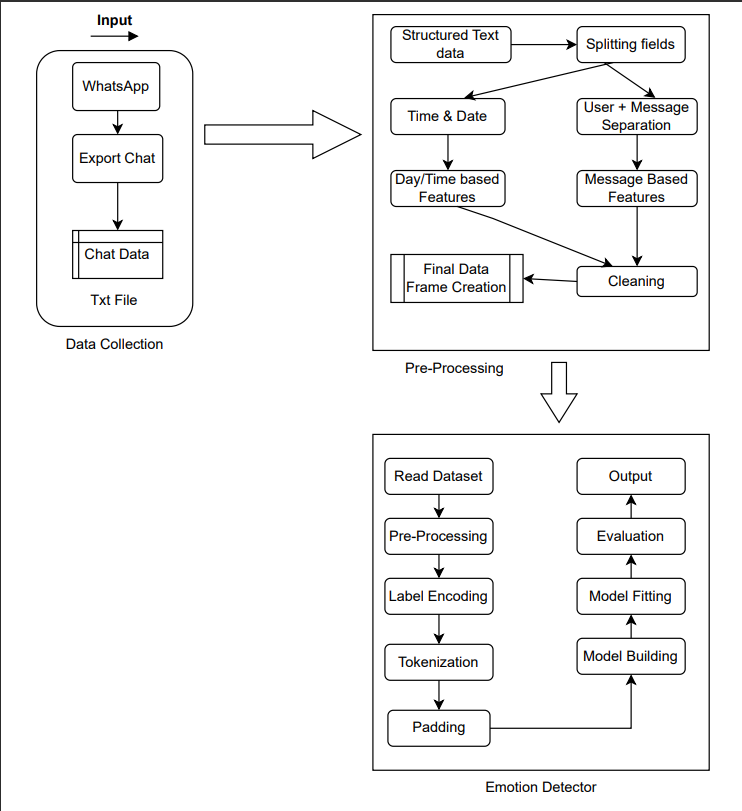
\includegraphics[width=\linewidth]{chapters/arcdesign.png}
  \caption{System architecture}
\end{figure}


\section{Module Description}
Here we provide detailed information about the modules of our system. That defines how our system works.
\begin{itemize}
\item Data collection
\item Pre-processing
\item FastText Word Vector Model
\item LSTM
\end{itemize}

\subsection{Data Collection}
To run our system at first we need a data set from where we can perform emotion detection. For our system we choose Whatsapp for our dataset. From a Whatsapp group we can easily collect our desire dataset. Whasapp export all chats in form of text file by default. It exports chats in a fixed pattern that is [Timestamp-Username-Messages]. There are also two options, we can export chats either with media or without media. Thus our system only suitable for text so we need chats without media.
 
To collect chat data from Whatsapp at first we have to open Whatsapp on phone. Then open an individual group or chat. Then click three dot from the right top corner of the screen. Here we found More option. Then click More option. After that click on Export Chat. That's how we can collect raw dataset.

\subsection{Pre-processing}
After export the chats we load it into the application to do this at first we have to extract all the information like time, date, day, user, messages etc. Then we have to remove stop words and punctuations. There are some major modules in preprocessing:
\begin{itemize}
\item \textbf{Splitting Fields:} We previously mentioned that the pattern of Whatsapp data is [Timestamp-Username-Messages]. So in this step the Timestamp is extracted from the chat using regular expression.

\item \textbf{Data frame creation:} After Timestamp and message are extracted the data frame is created. TO create the data frame pandas library is used.

\item \textbf{Date format conversion:} Whatsapp is installed locally in each device. That's why the data set will be in device's date format such as [DD/MM/YYYY, DD/MMM/YY, MM/DD/YYYY, MM/DD/YY etc]. But Python date format is YYYY/MM/DD. So here the custom date format is converted into Python's date format.

\item \textbf{Time format conversion:} Time is also present in custom format in each device just like date such as 12 hour format, 24 hour format. So in this step custom date formats are converted into a single date format which is 24 hour date format.
 
\item \textbf{Feature addition:} Here other meaningful information are extracted from all fields. For example Day, Date, Hour, Minute, Day Part, Period etc. has been extracted from timestamp. Similarly URLs, emojis, word count, media count etc. are also extracted from the messages part.
 
\item \textbf{Cleaning:} Here punctuations, stop words and unnecessary data are removed. 
\end{itemize}

\subsection{FastText Word Vector Model}
In sentiment evaluation word embedding techniques are considered as an important factor. FastText is a word embedding technique which is used in our system. Fasttext model is a extended version of word2vec model. Usual embadded technique uses word to build word embedding but Fasttext works one level deeper. It uses part of the word to build word embedding. For example the word, “normal” with n=3,the fastText representation of this word is ⟨nor,orm,rma,mal⟩, where the angular brackets indicatethe beginning and end of the word.

\subsection{LSTM}
LSTM stands for long short-term memory networks which is used in the field of Deep Learning.LSTM is a advanced version of recurrent neural networks (RNNs) that is design to learn long-term dependencies, especially in sequence prediction problems.

\subsubsection{Architecture of LSTM}
The role of an LSTM model is held by a memory cell known as
a cell state that maintains its state over time. The cell state is the horizontal line that runs through the top of the below diagram. Information can be added to or removed from the cell state in LSTM and is regulated by gates. These gates optionally let the information flow in and out of the cell. It contains a point-wise multiplication operation and a sigmoid neural net layer that assist the mechanism. The sigmoid layer gives out numbers between zero and one, where
zero means nothing should be let through, and one means everything should be let through.


\begin{figure}[h!]
  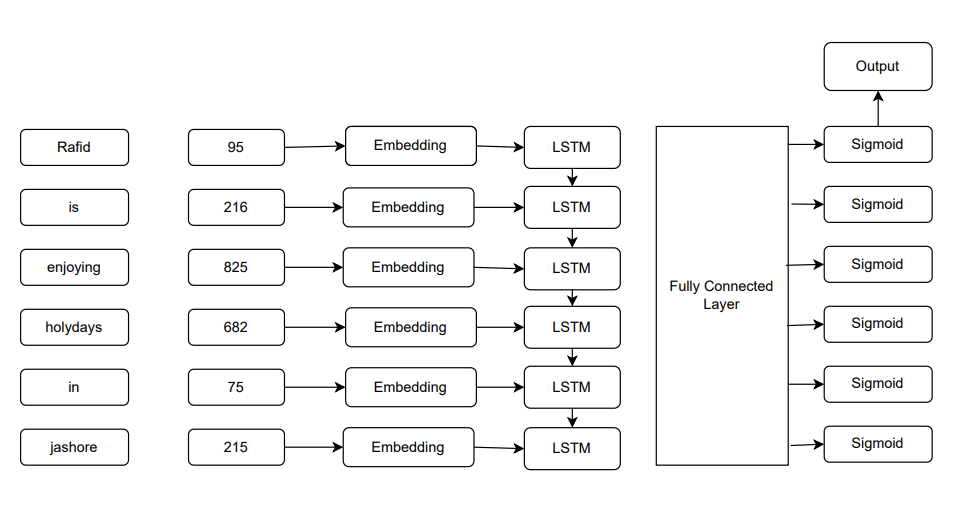
\includegraphics[width=\linewidth]{chapters/LSTM.png}
  \caption{LSTM architecture}
\end{figure}

There are mainly five layers in LSTM network. But layer an be added to improve the accuracy of the model. The five layers are:
\begin{itemize}
\item \textbf{Embedding Layer:} This Layer is responsible for converting word tokens into embedding of a specific size like 256, 512 etc. This layer maps a sequence of word indices to embedding vectors and learns the word embedding during training.
In this layer the word tokens are converted into embedding of a specific size like 256,512 etc. This layer also responsible for mapping a sequence of word indices to embedding vectors and learns the word embedding during training.

\item \textbf{LSTM Layer:}This layer sequentially process data and keep its hidden state through time. It keeps previous memory and process with current memory and decides whether to keep current memory or remain with old memory.
   
\item \textbf{Fully Connected Layer:} This layer indicates those layers where all inputs from one layer are connected to every unit of the next layer.

\item \textbf{Sigmoid Activation Layer:} This layer is responsible for converting all output values in the range of 0 to 1. It means it can either let no flow or complete flow of information throughout the gates.

\item \textbf{Output Layer:} Output layer is the final layer of the architecture. This layer is responsible for generating output which is obtained from sigmoid layer. The output formate is 2d array of real numbers where the first dimension indicates the number of samples given to the LSTM layer and second dimension is the dimensionality of the output space defined by the units
parameter in Keras LSTM implementation.
\end{itemize}






























